% Shared section: income, region and national well-being (method and results)
\subsection{Empirical strategy}\label{subsec:method_region}

For each well-being indicator $y$ and each income indicator $x$, I estimate three linear regressions across country-years $i$:
\begin{align}
    y_i &= \alpha_1 + \beta_1\, x_i + u_i \label{eq:income}\\
    y_i &= \alpha_2 + \gamma_2' R_i + e_i \label{eq:region}\\
    y_i &= \alpha_3 + \beta_3\, x_i + \gamma_3' R_i + \varepsilon_i \label{eq:both}
\end{align}
where $R_i$ is a vector of region dummies. Denoting $R^2_1$, $R^2_2$ and $R^2_3$ their coefficients of determination, the share of the variance explained by income alone is $R^2_1$. To compare income and region, I decompose $R^2_3$ between the two regressors following \citet{lindeman_introduction_1980} (LMG), i.e.\ using the Shapley value \citep{gromping_estimators_2007}. With two (groups of) regressors, the LMG contribution of income is the average of its contribution when entered first ($R^2_1$) and when entered second ($R^2_3 - R^2_2$). The \textit{share of explained variance due to income} is therefore
\begin{equation}
    s = \frac{R^2_1 + (R^2_3 - R^2_2)}{2\, R^2_3}, \label{eq:share}
\end{equation}
and region is the better predictor whenever $s < 50\%$.

Two features of this comparison could favor region. First, region has four degrees of freedom while log GDP has one. Second, the regions were not chosen blindly. To address the first concern, I report adjusted $R^2$ and, more directly relevant to the question of \textit{predictive} capacity, leave-one-country-out cross-validated $R^2$: each country's observations are predicted by a model estimated on all other countries, and the out-of-sample $R^2$ is one minus the ratio of the sum of squared prediction errors to the total sum of squares. To address the second concern, I report results for four alternative classifications. Other robustness checks include each WVS wave separately, weighting countries by their population, keeping only the last observation of each country, excluding the pandemic years 2020--2021, excluding imputed GDP values, using the previous vintage of GDP data (PPP in constant 2017 dollars), and excluding Latin America and Eastern Europe.

\subsection{Income explains a small share of national well-being in the WVS}\label{subsec:r2_income}

Figure~\ref{fig:satisfaction_gdp} plots mean life satisfaction against GDP per capita for all WVS country-years. The relationship is positive, but the dispersion at any given income level is large: countries with a GDP per capita around 10,000 dollars span most of the range of observed life satisfaction, from the former Soviet republics at the bottom to Latin American countries at the top. Log GDP per capita explains \RtwoSatisfiedMeanPPP\% of the variance of mean satisfaction.

\begin{figure}[htbp]
    \centering
    \caption{Mean life satisfaction vs.\ GDP per capita (PPP), WVS 1981--2022}\label{fig:satisfaction_gdp}
    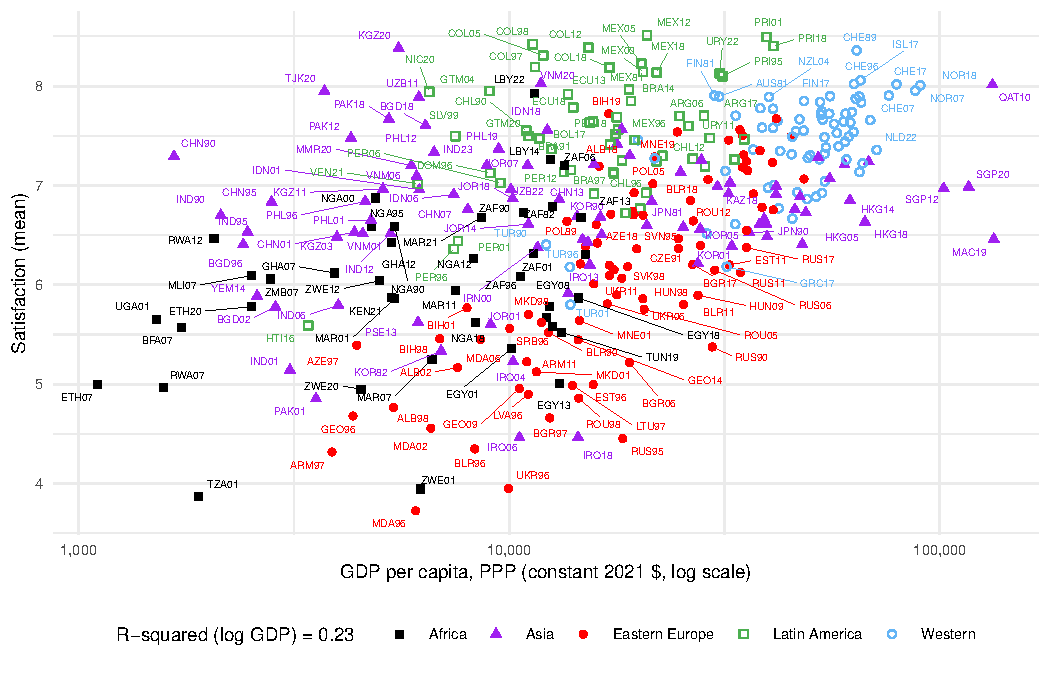
\includegraphics[width=.95\textwidth]{../figures/main/wvs_satisfied_mean_vs_gdp_ppp.pdf}
    \begin{minipage}{.95\textwidth}\footnotesize \textit{Note:} Each point is a country-year (label: ISO code and last two digits of the year). The legend gives the $R^2$ of the regression on log GDP per capita.\end{minipage}
\end{figure}

Table~\ref{tab:r2_income} generalizes this result to all indicators and income measures. On average over the eight indicators, log GDP per capita at PPP explains \meanRtwoIncomePPP\% of the variance, and the best-performing income measure (\bestIncome) explains \meanRtwoIncomeBest\%. The indicators are positively but imperfectly correlated (Appendix Table~\ref{tab:correlation}), and satisfaction-based indicators are better explained than happiness-based ones: log GDP explains \RtwoHappinessMeanPPP\% of the variance of mean happiness and essentially none of the share of \textit{Very happy} people, whose slope with respect to log GDP is statistically indistinguishable from zero (slope \slopeVeryHappy, $p = \pVeryHappy$; Appendix Table~\ref{tab:slopes}). This confirms the observation of \citet{deaton_income_2008} and \citet{inglehart_development_2008} that income is more closely related to life evaluation than to happiness. By contrast, region alone explains \meanRtwoRegion\% of the variance on average (last column).

\begin{table}[htbp]
    \centering
    \caption{Share of the variance of national well-being explained by income alone ($R^2$), WVS 1981--2022}\label{tab:r2_income}
    \begin{adjustbox}{max width=\textwidth}
    \begin{tabular}{lcccccccc}
\toprule
Well-being indicator & \multicolumn{2}{c}{log GDP p.c.} & Sextile & \multicolumn{4}{c}{Income cluster} \\ & PPP & nominal & PPP & $k$=5 PPP & $k$=6 PPP & $k$=7 PPP & $k$=7 nominal & Region \\
\midrule
Happy & 0.13 & 0.18 & 0.20 & 0.19 & 0.19 & 0.20 & 0.23 & 0.36 \\
Very Happy & 0.00 & 0.00 & 0.03 & 0.02 & 0.03 & 0.04 & 0.03 & 0.35 \\
Very Unhappy & 0.06 & 0.09 & 0.12 & 0.11 & 0.13 & 0.13 & 0.14 & 0.16 \\
V. Happy -- V. Unhappy & 0.00 & 0.01 & 0.05 & 0.03 & 0.04 & 0.05 & 0.04 & 0.36 \\
Happiness (mean) & 0.04 & 0.07 & 0.10 & 0.08 & 0.09 & 0.10 & 0.10 & 0.38 \\
Satisfaction (mean) & 0.20 & 0.26 & 0.21 & 0.19 & 0.19 & 0.21 & 0.26 & 0.48 \\
Satisfied & 0.28 & 0.35 & 0.30 & 0.28 & 0.28 & 0.30 & 0.35 & 0.45 \\
Happy + Satisfied & 0.25 & 0.32 & 0.28 & 0.27 & 0.27 & 0.29 & 0.33 & 0.46 \\
\midrule
Mean & 0.12 & 0.16 & 0.16 & 0.15 & 0.15 & 0.17 & 0.19 & 0.37 \\
Max & 0.28 & 0.35 & 0.30 & 0.28 & 0.28 & 0.30 & 0.35 & 0.48 \\
\bottomrule
\end{tabular}

    \end{adjustbox}
    \begin{minipage}{\textwidth}\footnotesize \textit{Note:} $R^2$ of the regression of each well-being indicator (rows) on each income indicator (columns), over \nWVSCountryYears WVS country-years (a few with missing GDP are excluded). The last column gives the $R^2$ of the regression on region dummies.\end{minipage}
\end{table}

\subsection{Region predicts national well-being better than income in the WVS}\label{subsec:region_wvs}

Table~\ref{tab:share_income} reports the share of explained variance due to income, $s$, for each indicator and income measure. It is below 50\% in all cases: on average, the best income measure accounts for \meanShareIncomeBest\% of the variance explained jointly by income and region. The first split of a regression tree using log GDP and region as candidate variables is on region for \treeRegionFirst out of 8 indicators.

\begin{table}[htbp]
    \centering
    \caption{Share of explained variance due to income rather than region (LMG), WVS 1981--2022}\label{tab:share_income}
    \begin{adjustbox}{max width=\textwidth}
    \begin{tabular}{lccccccc}
\toprule
Well-being indicator & \multicolumn{2}{c}{log GDP p.c.} & Sextile & \multicolumn{4}{c}{Income cluster} \\ & PPP & nominal & PPP & $k$=5 PPP & $k$=6 PPP & $k$=7 PPP & $k$=7 nominal \\
\midrule
Happy & 0.22 & 0.29 & 0.31 & 0.30 & 0.30 & 0.32 & 0.34 \\
Very Happy & 0.00 & 0.01 & 0.07 & 0.05 & 0.08 & 0.10 & 0.07 \\
Very Unhappy & 0.22 & 0.31 & 0.41 & 0.38 & 0.43 & 0.44 & 0.45 \\
V. Happy -- V. Unhappy & 0.01 & 0.02 & 0.09 & 0.06 & 0.09 & 0.11 & 0.08 \\
Happiness (mean) & 0.07 & 0.11 & 0.15 & 0.13 & 0.15 & 0.16 & 0.15 \\
Satisfaction (mean) & 0.25 & 0.30 & 0.25 & 0.23 & 0.23 & 0.25 & 0.30 \\
Satisfied & 0.35 & 0.41 & 0.36 & 0.34 & 0.35 & 0.37 & 0.41 \\
Happy + Satisfied & 0.31 & 0.38 & 0.35 & 0.33 & 0.34 & 0.35 & 0.39 \\
\midrule
Mean & 0.18 & 0.23 & 0.25 & 0.23 & 0.25 & 0.26 & 0.28 \\
Max & 0.35 & 0.41 & 0.41 & 0.38 & 0.43 & 0.44 & 0.45 \\
\bottomrule
\end{tabular}

    \end{adjustbox}
    \begin{minipage}{\textwidth}\footnotesize \textit{Note:} Share of the $R^2$ of Equation~\eqref{eq:both} attributed to income by the LMG (Shapley) decomposition, Equation~\eqref{eq:share}. Values below 0.5 indicate that region is the better predictor.\end{minipage}
\end{table}

The result is not an artifact of the larger number of parameters of the region model. Out of sample, region predicts better than income for every indicator (Table~\ref{tab:cv}): for mean satisfaction, the leave-one-country-out $R^2$ is \cvRegionSatisfiedMean with region against \cvIncomeSatisfiedMean with log GDP. For several happiness indicators, income has no out-of-sample predictive power at all (negative cross-validated $R^2$).

\begin{table}[htbp]
    \centering
    \caption{Out-of-sample predictive capacity: leave-one-country-out cross-validated $R^2$}\label{tab:cv}
    \begin{adjustbox}{max width=\textwidth}
    \begin{tabular}{llccccc}
\toprule
Data & Indicator & Obs. & log GDP PPP & Best income variable & Region & log GDP PPP + Region \\
\midrule
WVS, all waves & Happy & 302 & 0.11 & 0.17 & 0.31 & 0.36 \\
WVS, all waves & Very Happy & 302 & -0.03 & -0.06 & 0.29 & 0.29 \\
WVS, all waves & Very Unhappy & 302 & 0.05 & 0.09 & 0.11 & 0.12 \\
WVS, all waves & V. Happy -- V. Unhappy & 302 & -0.02 & -0.05 & 0.30 & 0.29 \\
WVS, all waves & Happiness (mean) & 302 & 0.02 & 0.03 & 0.33 & 0.33 \\
WVS, all waves & Satisfaction (mean) & 302 & 0.18 & 0.19 & 0.44 & 0.51 \\
WVS, all waves & Satisfied & 302 & 0.26 & 0.30 & 0.42 & 0.53 \\
WVS, all waves & Happy + Satisfied & 300 & 0.23 & 0.28 & 0.42 & 0.51 \\
\midrule
WVS, last obs. per country & Happy & 108 & 0.05 & 0.10 & 0.24 & 0.26 \\
WVS, last obs. per country & Very Happy & 108 & -0.01 & -0.04 & 0.25 & 0.24 \\
WVS, last obs. per country & Very Unhappy & 108 & 0.04 & 0.04 & 0.05 & 0.07 \\
WVS, last obs. per country & V. Happy -- V. Unhappy & 108 & -0.02 & -0.06 & 0.25 & 0.24 \\
WVS, last obs. per country & Happiness (mean) & 108 & -0.04 & -0.04 & 0.26 & 0.24 \\
WVS, last obs. per country & Satisfaction (mean) & 108 & 0.13 & 0.12 & 0.36 & 0.40 \\
WVS, last obs. per country & Satisfied & 108 & 0.22 & 0.23 & 0.34 & 0.42 \\
WVS, last obs. per country & Happy + Satisfied & 108 & 0.18 & 0.20 & 0.36 & 0.42 \\
\midrule
Gallup, all years (2006--23) & Satisfaction (mean) & 2344 & 0.61 & 0.66 & 0.49 & 0.68 \\
Gallup, all years (2006--23) & Satisfied & 2344 & 0.65 & 0.72 & 0.52 & 0.72 \\
Gallup, all years (2006--23) & Unsatisfied (0/1--4) & 2344 & 0.63 & 0.65 & 0.48 & 0.68 \\
\midrule
Gallup, last obs. per country & Satisfaction (mean) & 167 & 0.60 & 0.58 & 0.45 & 0.64 \\
Gallup, last obs. per country & Satisfied & 167 & 0.65 & 0.68 & 0.52 & 0.70 \\
Gallup, last obs. per country & Unsatisfied (0/1--4) & 167 & 0.65 & 0.60 & 0.48 & 0.67 \\
\midrule
WHR, 2023--25 average & Satisfaction (mean) & 147 & 0.62 & 0.60 & 0.52 & 0.69 \\
\bottomrule
\end{tabular}

    \end{adjustbox}
    \begin{minipage}{\textwidth}\footnotesize \textit{Note:} Each country's observations are predicted with a model estimated on all other countries. Cross-validated $R^2 = 1 - \sum (y - \hat y_{\text{out-of-sample}})^2 / \sum (y - \bar y)^2$; it can be negative when a model predicts worse than the overall mean.\end{minipage}
\end{table}

Table~\ref{tab:robustness} summarizes \nSpecsWVS estimates (indicator $\times$ income measure $\times$ specification) using the WVS. Region is the better predictor in \shareRegionBetterWVS\% of them (\shareRegionBetterWVSbest\% when restricting to the best income measure). The result holds in each wave except wave 4 (1999--2004, 40 countries), where income and region perform similarly; when countries are weighted by population; when keeping one observation per country; without the pandemic years; without imputed GDP values; with the previous vintage of GDP data; and with the six-region or the UN sub-region classifications.

\begin{table}[htbp]
    \centering
    \caption{Robustness: income vs.\ region across specifications and datasets}\label{tab:robustness}
    \begin{adjustbox}{max width=\textwidth}
    \begin{tabular}{lccccccccc}
\toprule
Specification & Obs. & Countries & \multicolumn{2}{c}{$R^2$ income} & $R^2$ region & \multicolumn{3}{c}{Share of explained variance due to income} & Region better \\ & & & log PPP & best & & log PPP & best & adj. $R^2$ & (share of cases) \\
\midrule
WVS, all waves & 302 & 108 & 0.12 & 0.19 & 0.37 & 0.18 & 0.28 & 0.22 & 1.00 \\
WVS, waves 1--2 (1981--91) & 26 & 21 & 0.07 & 0.43 & 0.58 & 0.09 & 0.40 & 0.10 & 1.00 \\
WVS, wave 3 (1995--99) & 55 & 55 & 0.16 & 0.33 & 0.65 & 0.14 & 0.28 & 0.18 & 1.00 \\
WVS, wave 4 (1999--2004) & 40 & 40 & 0.19 & 0.31 & 0.33 & 0.27 & 0.47 & 0.47 & 0.43 \\
WVS, wave 5 (2004--09) & 58 & 58 & 0.21 & 0.35 & 0.49 & 0.22 & 0.38 & 0.23 & 0.98 \\
WVS, wave 6 (2010--16) & 60 & 60 & 0.08 & 0.22 & 0.27 & 0.14 & 0.41 & 0.19 & 0.96 \\
WVS, wave 7 (2017--22) & 64 & 64 & 0.07 & 0.13 & 0.26 & 0.20 & 0.31 & 0.14 & 1.00 \\
WVS, wave 7 w/o 2020--21 & 45 & 45 & 0.06 & 0.22 & 0.31 & 0.14 & 0.41 & 0.14 & 0.95 \\
WVS, population-weighted & 302 & 108 & 0.10 & 0.19 & 0.23 & 0.24 & 0.44 & 0.33 & 0.84 \\
WVS, last obs. per country & 108 & 108 & 0.10 & 0.18 & 0.33 & 0.18 & 0.32 & 0.21 & 0.96 \\
WVS, no GDP imputation & 283 & 104 & 0.12 & 0.19 & 0.38 & 0.17 & 0.28 & 0.21 & 1.00 \\
WVS, GDP PPP 2017 \$ (old) & 302 & 108 & 0.13 & 0.19 & 0.37 & 0.19 & 0.28 & 0.22 & 1.00 \\
WVS, w/o Latin Am. \& E. Europe & 185 & 68 & 0.16 & 0.27 & 0.18 & 0.34 & 0.68 & 0.54 & 0.27 \\
WVS, 6 regions & 302 & 108 & 0.12 & 0.19 & 0.35 & 0.18 & 0.28 & 0.22 & 1.00 \\
WVS, World Bank regions (7) & 302 & 108 & 0.12 & 0.19 & 0.22 & 0.31 & 0.43 & 0.38 & 0.64 \\
WVS, continents (5) & 302 & 108 & 0.12 & 0.19 & 0.20 & 0.34 & 0.46 & 0.41 & 0.54 \\
WVS, UN sub-regions & 302 & 108 & 0.12 & 0.19 & 0.40 & 0.20 & 0.29 & 0.25 & 1.00 \\
\midrule
Gallup, all years (2006--23) & 2344 & 167 & 0.42 & 0.48 & 0.42 & 0.46 & 0.51 & 0.49 & 0.31 \\
Gallup, last obs. per country & 167 & 167 & 0.42 & 0.44 & 0.41 & 0.44 & 0.48 & 0.45 & 0.37 \\
Gallup, last obs., WVS countries & 105 & 105 & 0.43 & 0.46 & 0.42 & 0.46 & 0.49 & 0.47 & 0.37 \\
Gallup, last obs., 6 regions & 167 & 167 & 0.42 & 0.44 & 0.42 & 0.43 & 0.46 & 0.44 & 0.41 \\
Gallup, last obs., WB regions & 167 & 167 & 0.42 & 0.44 & 0.38 & 0.47 & 0.50 & 0.48 & 0.29 \\
WHR, 2023--25 average & 147 & 147 & 0.63 & 0.63 & 0.55 & 0.56 & 0.56 & 0.56 & 0.00 \\
\bottomrule
\end{tabular}

    \end{adjustbox}
    \begin{minipage}{\textwidth}\footnotesize \textit{Note:} Averages over well-being indicators (8 for the WVS; 7 satisfaction indicators for Gallup; mean ladder for the WHR). ``Best'' refers to the income measure with the highest average $R^2$ in the main WVS specification (\bestIncome). ``Region better'' is the share of indicator $\times$ income-measure combinations for which $s < 0.5$.\end{minipage}
\end{table}

\subsection{Where the region advantage comes from}\label{subsec:region_limits}

Three results qualify this conclusion. First, the advantage of region is driven by two well-known ``anomalies'': Latin America, happier than its income would predict \citep{graham_paradox_2009,rojas_handbook_2016}, and the former Eastern Bloc, unhappier \citep{guriev_unhappiness_2009}. Excluding these two regions, region is the better predictor in only \shareRegionBetterNoLatamEE\% of cases. Second, the result depends on the granularity and design of the classification: with continents or World Bank regions, which do not isolate Latin America or the former Eastern Bloc, region is better in \shareRegionBetterContinents\% and \shareRegionBetterWB\% of cases, respectively. Third, and most importantly, the conclusion does not carry over to Gallup data. In Gallup's latest observation for each of \nGallupCountries countries, log GDP explains \RtwoGallupMeanPPP\% of the variance of the mean ladder, against \RtwoGallupRegion\% for region, and income accounts for \shareIncomeGallupMean\% of the explained variance (Appendix Table~\ref{tab:share_gallup}). Over all Gallup specifications, region is the better predictor in only \shareRegionBetterGallup\% of cases, mostly for indicators of the upper tail of the distribution (shares answering 9--10 or 10), which are almost unrelated to income. With the latest WHR data (2023--2025), log GDP explains \RtwoWHRPPP\% of the variance of the ladder against \RtwoWHRRegion\% for region.

The relation between GDP and well-being is thus much weaker in the WVS than in Gallup. The same holds when restricting both datasets to the \nCommon country-years observed by both surveys: the $R^2$ of mean life evaluation on log GDP is \RtwoCommonGallup in Gallup and \RtwoCommonWVS in the WVS. Whether ``GDP is a poor predictor of national well-being'' therefore depends on which of the two datasets one trusts.

\subsection{Other correlates and within-country evidence}\label{subsec:correlates}

What do regions capture? Appendix Table~\ref{tab:correlates} decomposes the variance of mean satisfaction among income, region and one additional country-level variable from the WVS. The average perceived freedom of choice and control over one's life (``how much freedom of choice and control you feel you have over the way your life turns out'') alone explains \RtwoFreedomSatisfaction\% of the variance of mean satisfaction; in a Shapley decomposition with income and region, it accounts for \shapleyFreedom percentage points, against \shapleyFreedomRegion for region and \shapleyFreedomIncome for income. This variable is itself a subjective evaluation, so this correlation should not be read causally, but it suggests that non-material dimensions of life are central to regional differences \citep{inglehart_development_2008}. Tolerance of homosexuality (\RtwoTolerance\%), the importance of God (\RtwoGod\%) and GDP growth over the previous five years (\RtwoGrowth\%) explain much less.

Finally, the cross-sectional relation should not be confused with the relation over time. Within countries (country fixed effects, \nWithin observations from countries surveyed at least twice), mean satisfaction increases with log GDP per capita, with a slope of \withinSlopeSatisfiedMean per unit of $\log_{10}$ GDP (i.e.\ per tenfold increase), larger than the cross-sectional slope (\crossSlopeSatisfiedMean), and even the share of \textit{Very happy} people increases (slope \withinSlopeVeryHappy, $p = \pWithinVeryHappy$). Income growth explains \withinRtwoSatisfiedMean of the within-country variance (Appendix Table~\ref{tab:within}). These within-country associations are consistent with \citet{stevenson_economic_2008} and \citet{sacks_new_2012} rather than with a strict version of the Easterlin paradox \citep{easterlin_does_1974,easterlin_happiness_2010}, although they may reflect common shocks (e.g.\ transition recessions) rather than the effect of income per se.

\subsection{What are the happiest countries?}\label{subsec:happiest}

Rankings of countries depend on the indicator. Taking, for each indicator and each wave (and all waves combined), the happiest country-year, \happiestFirst appears most often (\happiestFirstN times out of \nHappiestCells), followed by \happiestSecond (\happiestSecondN) and \happiestThird (\happiestThirdN) (Appendix Table~\ref{tab:happiest}). The happiest country-years are Western (\happiestRegionWestern), Latin American (\happiestRegionLatinAmerica), Asian (\happiestRegionAsia) or African (\happiestRegionAfrica). The richest countries are thus not necessarily the happiest: the link between income and well-being seems to be that rich countries rarely experience low well-being, rather than that they reach the highest levels.
